

\section{Study 1: Understanding Explanations and Feedback with a Low Quality Model} 
With a crowdsourced, between-subjects experiment, we explored how explanations and support for feedback affect satisfaction and expectation of change with a low quality model. 
%We use crowd workers, as we are interested in end users without ML expertise.

\subsection{Method}
Simple models and tasks are a useful starting point to examine the intersection of explanations and feedback.
Therefore, in this study, participants reviewed a simple text classification
model's predictions with or without explanations and with one of three options for providing user feedback to the model: no feedback, correcting or confirming the model's predictions (instance-level feedback), or suggesting important words to the model (feature-level feedback). 

\paragraph{Task, Model, Feedback, and Explanations}
We chose a simple model and task that a large population of non-ML experts could use to interact with and evaluate ML models.
%
Specifically, we chose text classification as it is prevalent in real-world use cases, such as document recommendation and search. Borrowing from prior work~\cite{Kulesza2015PrinciplesLearning, Settles2011ClosingInstances}, we used a text classification algorithm to predict the category of emails from a data set of 2,000 ``hockey'' and ``baseball'' emails from the 20 Newsgroups corpus~\cite{Lang1995NewsWeeder:Netnews}. 
%and used a text classification algorithm to predict whether each email is about ``hockey'' or ``baseball''. 

% classifier and model specifics
%Like prior work~\cite{Kulesza2015PrinciplesLearning}, 
Specifically, we used a Na\"ive Bayes model with unigram features~\cite{Lewis1998NaiveBayesatRetrieval}---the multinomial Na\"ive Bayes (\texttt{MultinomialNB}) classifier from the \texttt{scikit-learn} library~\cite{Pedregosa2011Scikit-learn:Python}.
%
We performed standard pre-processing procedures on the emails.\footnote{We removed non-alphabetical characters, lowercased all words, tokenized by whitespace, and dropped \textit{From:} lines from the emails to prevent the model from training on email addresses.} For this experiment, we trained the classifier on $16$ (of the $1197$) labeled training emails (eight per class), with $76.5\%$ classification accuracy on the $796$ emails in the test set.

% task overview
The participants were to imagine that they had been assigned to sort their boss's email inbox. They were told that they would evaluate a ML model designed to help them. Would it be worthwhile to add the model to their workflow?

\newcommand{\FigureMethodInteractPhase}{
\begin{figure}[t]
    \begin{center}
    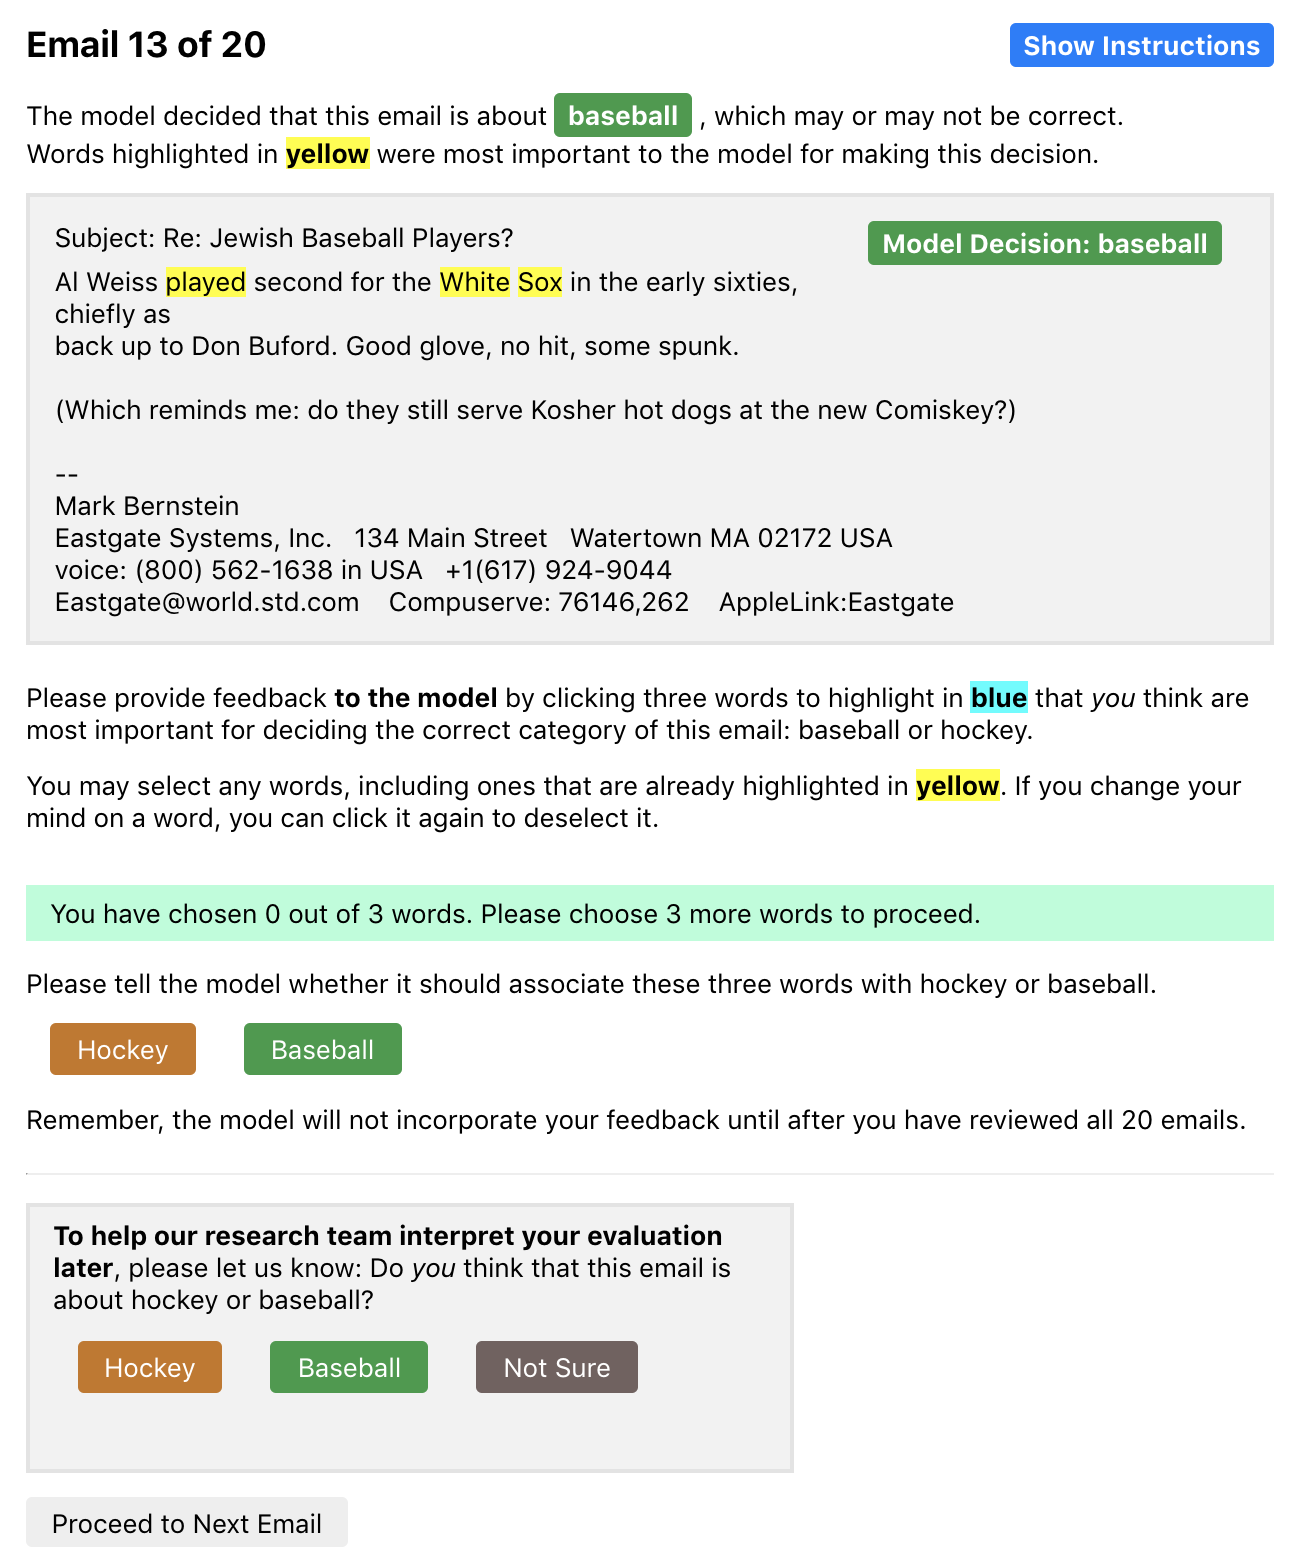
\includegraphics[width=.4\textwidth]{2020_chi_explanation/figures/p20_interact_email13.png}
    \end{center}
    \caption{Screenshot of an email in the ``interaction phase'' for a participant in the feature-level feedback and explanation condition (E-F).}
    \vspace{-10pt}
    \label{fig:interact_phase}
\end{figure}
}

\newcommand{\FigureMethodEvalPhase}{
\begin{figure}[t]
    \begin{center}
    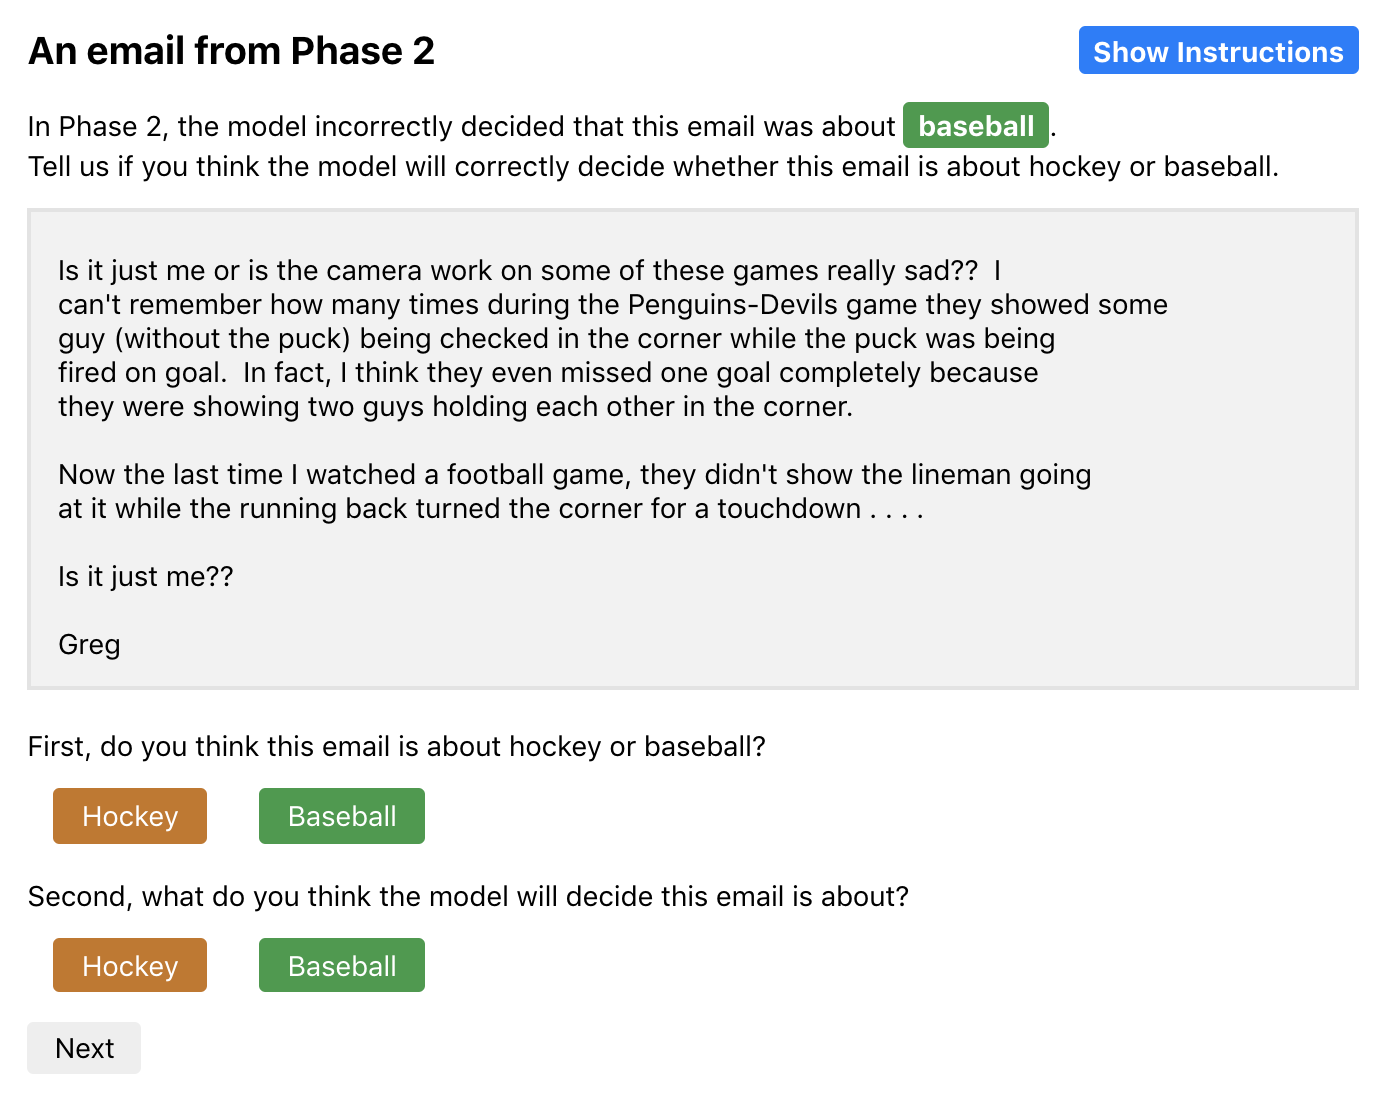
\includegraphics[width=.4\textwidth]{2020_chi_explanation/figures/p36_evaluate_test4.png}
    \end{center}
    \caption{Screenshot of an email in the ``evaluation phase,'' where participants predicted how the model would label an email that it had previously labeled incorrectly in the ``interaction phase.''}
    \label{fig:eval_phase}
\end{figure}
}

For this task, we built an interface where participants review emails with the model's ``hockey'' or ``baseball'' prediction (Figure~\ref{fig:interact_phase}).\footnote{https://github.com/rococode/bh-classifier} The interface either displays an explanation of the model's prediction (or not) and supports either no user feedback, feature-level feedback, or instance-level feedback. 

% feedback and explanations
Our explanations tell users what the model regards as important for prediction: we highlight the three words that are most influential to the class prediction for a given email, $abs(p(w \g baseball) - p(w \g hockey))$. This method is purposefully simple and truthful to the classifier's methodology, two guidelines for good explanations~\cite{Kulesza2013TooModels, Narayanan2018HowExplanation}. Additionally, we choose exactly three words as explanations should include \textit{sufficient}, but not \textit{extra}, low-level context~\cite{Rosenthal2010TowardsData}. 

For \textit{instance-level} feedback, participants correct or confirm each classification by telling the model whether the email is about ``hockey'' or ``baseball.'' For \textit{feature-level} feedback, participants tell the model what should be important by providing the top three words they think would be most useful in classifying a given email and specifying the class with which those words should be associated. %This feedback is not incorporated into the model at any point during the task.

\subsubsection{Participants}
We recruited $180$ unique participants ($77$ male, $102$ female, and one unspecified) from Mechanical Turk,\footnote{http://mturk.com} requiring participants with the ``Masters'' qualification, located in the United States, and having completed more than 500  HITs with approval rate $98\%$ or higher. 
Two participants were 18--24 years old, 62 aged 25--34, 60 aged 35--44, 30 aged 45--54, 22 aged 55--64, and 4 aged 65--74. Participants rated their prior knowledge on five-point Likert scales for ML (65 had none, 67 had a little, 44 had some, four had a lot, and none had expert), hockey (15 had none, 78 had a little, 65 had some, 18 had a lot, and four had expert), and baseball (two had none, 43 had a little, 68 had some, 57 had a lot, and 10 had expert).

\subsubsection{Procedure}
Remote study sessions took on average $22.6$ minutes~($SD=15.3$). Participants completed three phases: (1) introduction, (2) ``interaction'' with the model, and (3) ``evaluation'' of the model. To motivate quality work, participants were told that at least the top $50\%$ of participants would be given a $\$2$ bonus based on the thoroughness of their evaluations; unbeknownst to them, all ultimately received the bonus. 

\FigureMethodInteractPhase

% Task and emails description
During the ``interaction phase'', participants reviewed 20 emails,\footnote{We randomly select these 20 emails for Study 1, requiring even distribution between hockey and baseball predictions, five incorrect and 15 correct, and that emails be between 30 and 120 characters; we use the same set of emails for Study~2.} in randomized order per participant. 
%
The model provided a prediction (``hockey'' or ``baseball'') for each email. Participants in the \textit{explanation} conditions saw the model's top three words highlighted. Participants in the \textit{instance-level feedback} conditions corrected or confirmed the model's prediction for each email, and participants in the \textit{feature-level feedback} conditions specified their three important words for predicting the correct class. To determine whether participants knew the correct labels, as this might affect their evaluation, all participants also told us (not the model) the correct email label, with an option for ``not sure''. 

\FigureMethodEvalPhase

During the ``evaluation phase'', participants responded to closed- and open-ended questions on satisfaction and model change expectations, including rating scales as shown in Table~\ref{tab:subjective_measures} paired with the follow up of ``Why do you feel this way''.\footnote{An additional two rating scales of acceptable accuracy and expectations of learning are not reported on here due to space constraints and not being as directly related to our research questions.} After these questions, participants were shown four ``evaluation'' emails and asked to predict how the model would classify them (Figure~\ref{fig:eval_phase}). These emails included two of the 20 from the ``interaction phase'' and two new ones that were similar to emails in the first 20, as measured by cosine similarity~\cite{Huang2008SimilarityClustering}. For each email type (repeat or similar), we selected one that was previously labeled correctly and one that was previously labeled incorrectly by the model. These four emails allowed us to assess whether participants would expect the model's labels to change following the ``interaction phase''.

Importantly, feature- and instance-level feedback was \textbf{not} incorporated into the model during the ``interaction phase''; we reminded the feature- and instance-level participants of this with each email. This design choice isolates perceptions of explanations and feedback from how well the model incorporated that feedback.
%, such as introducing issues of unpredictable model updates. 
Instead, we told these participants that their feedback would be incorporated into the model \textit{after} they had reviewed all 20 emails, so they would expect an updated model for the ``evaluation phase''.\footnote{However, we never incorporate feedback during the study protocol, but users were unaware as we did not show model predictions or explanations during the ``evaluation phase.''}

\subsubsection{Study Design}
This study used a 2$\times$3 between-subjects experimental design, with factors of \textit{Explanation}---feature (E), none (N)---and \textit{Feedback}---feature (F), instance (I), none (N). An equal number of participants were randomly assigned to each condition.

\begin{table}[t!]
    \scriptsize
    \begin{center}
    \rowcolors{2}{gray!25}{white}
    \begin{tabular}{p{1.5cm} p{6.5cm}}
        \toprule
        Measure & Statement \\
        \midrule
        frustration & ``I would feel frustrated if I were to use this model to automatically sort my boss's emails''\\
        trust & ``I would trust this model to correctly categorize my boss's emails that are about hockey or baseball''\\
        accuracy & ``The model is able to distinguish between hockey and baseball emails''\\
        understanding & ``I understand how this model makes decisions''\\
        acceptance & ``I would use this model to help me sort my boss's emails''\\
        feedback importance & ``If I were to use this model, it would be important to have the ability to provide feedback to improve it''\\
        expected change & ``If the model were now shown another set of emails, how well do you think it would categorize them?''\\
        \bottomrule
    \end{tabular}
    \end{center}
    \caption{Seven-point rating scale statements for seven subjective measures. All are on a scale from \emph{strongly disagree} to \emph{strongly agree} aside from expected change, which is from \emph{much worse} to \emph{much better.}}
    \vspace{-10pt}
    \label{tab:subjective_measures}
\end{table}

\subsubsection{Measures and Hypotheses}
We report on seven main subjective measures, collected using seven-point rating scales (Table~\ref{tab:subjective_measures}): three \textit{user satisfaction} measures (frustration, trust, model acceptance), three \textit{user perception} measures (expected model improvement, perceived model accuracy, perceived understanding of how the model works), and \textit{desire to provide feedback} (feedback importance). 

While we explore the effects of feedback and explanation on user satisfaction in general, our primary user satisfaction hypothesis relates to \textbf{frustration}, as we hypothesize that users are frustrated without the ability to fix model errors exposed by explanations.

\begin{itemize*}
    \item \textbf{H1.1}: Feedback (instance- or feature-level) reduces frustration compared to no feedback.
    \item \textbf{H1.2}: Explanations without feedback increase frustration compared to no explanation without feedback. 
\end{itemize*}

While prior work has explored effects of explanation on mental models and perceptions of quality~\cite{Bilgic2005ExplainingPromotion,Lim2009WhySystems}, we explore a new concept, \textbf{expected improvement}, or how users expect ML models to improve with or without explicit feedback. %, as well as the level of feedback (instance or feature). 
Intuitively, providing feedback should increase this expectation. Based on human behavior~\cite{Siegler2009MicrogeneticSelf-explanation}, we also hypothesize that explanations might suggest a model is being introspective and could therefore \textit{learn from its mistakes}. 

\begin{itemize*}
    \item \textbf{H2.1}: Feedback (instance- or feature-level) increases the user's expectation that the model will improve compared to no feedback.
    \item \textbf{H2.2}: Explanations increase the user's expectation that the model will improve compared to no explanation. 
\end{itemize*}

\subsubsection{Data and Analysis}
After disqualifying one participant who only filled out the demographics survey and another who skipped part of the post-task survey, our dataset includes 178 participants. We used separate 2$\times$3 (\textit{Explanation}$\times$\textit{Feedback}) ANOVAs with Aligned Rank Transforms for each main subjective measure---a test more appropriate for Likert scale data than a standard ANOVA~\cite{Wobbrock2011TheProcedures}. For significant main effects of feedback we used post-hoc Wilcoxon rank sum tests with continuity correction and Holm-Bonferroni adjustments. We report on all significant results, including pairwise comparisons.

We qualitatively coded the open-ended responses related to our primary measures: frustration and expected improvement.
%
Two annotators individually read a subset of the responses to identify emergent codes, followed by a discussion period to generate a codebook.
%
Then, the two annotators independently coded a random subset of 20 of the 178 responses; agreement was scored using Cohen's $\kappa$: $\kappa=.93$ (raw agreement: 95\%) for frustration responses and $\kappa=.88$ (90\%) for expected improvement responses.
%
We refer to participants in this experiment with a lower quality model as LP1--LP178.


